\documentclass[11pt]{article}
\usepackage{etex}
\usepackage{amssymb}
\usepackage[margin=.8in]{geometry}
\usepackage{amsmath,graphicx}
\usepackage{algorithm}
\usepackage[usenames,dvipsnames]{color}
\usepackage{algorithmicx}
\usepackage{algpseudocode}
\usepackage{alphalph}
\usepackage{listings}
\usepackage{float}
\usepackage{caption}
\usepackage{amsmath}
\usepackage{subcaption}
\usepackage{tabularx}
\usepackage{framed}
\usepackage{tabu}
\usepackage{booktabs}
\usepackage{tikz}
\usepackage[stable]{footmisc}
\usepackage{titlesec}
\usepackage{setspace}
 \usepackage{alltt} 
\usepackage{hyperref}
\usepackage{pgfplots}

\newcommand{\bt}[1]{\textbf{#1}}    
   
  \begin{document}
  \title{CS691CL - Computational Linguistics: Syntax and Semantics \\ Final Project Report \\ \vspace{1cm} \emph{Document Similarity Measures \\ Utilizing Syntactics and Semantics \\ as well as Embeddings}}
  \author{Nicholas Monath,  Klim Zaporojets, Niklas Shulze}
  \maketitle
  
  
  
\section{Introduction}

There is no shortage of online databases of documents containing valuable information, but there is a need for more tools to organize this data to provide users a more accessible interface than a standard keyword search. Providing solutions to this problem of information overload has been the focus of years of research in information retrieval, natural language processing and machine learning in general. In particular, much work has been done on defining document similarity measures, which determine the relatedness of two documents based on their text content. Typical approaches to this problem are based in word usage statistics and are not able to capture the essence of a text, as the syntactic and semantic relationships of the words are disregarded. In this project, we will make use of dependency parsing and automatic semantic role labeling to extract syntactically and semantically related phrases from text. Using these phrases, we hope to create a more robust document representation and similarity measure than the traditional approaches. 

We would like to apply our proposed document similarity measure to the problem of identifying relatedness between scientific research papers. The similarity of scientific research papers is a less studied problem than document similarity in general and a robust measure is in high demand \cite{Hurtado2013}. Such a measure would be useful in both research paper recommender systems and search engines. 

The rest of this document is organized as follows: a review of related work done in this field and explanation of how our work differs from this previous research; our proposed approach to defining a document similarity measure; and an explanation of our proposed experiments.

\section{Related Work} \label{sec:RelatedWork}

Document similarity is a much studied problem in the field of information retrieval with a wide range of applications, such as document classification and clustering, searching in large unorganized datasets, and recommendation systems. The problem of document similarity extends beyond the measurement of relatedness of \emph{unstructured} documents containing only text to \emph{structured} documents, which contain hyperlinks and other annotations \cite{Manning2008}. 

The most common approach to unstructured text document similarity is a vector space, statistics based method known as the  \emph{bag-of-words} approach. The details of this approach are represented as a foundation for our model in Section \ref{sec:TraditionalApproaches}. Work in \cite{Huang2008} shows the effectiveness of this simple representation on a number of datasets in the problem of document clustering. Another common technique is the representation of documents with a \emph{language model}. First presented in \cite{Ponte1998}, language models make the assumption that the collection of individual terms in a document is a sample from a probability distribution. This approach is particularly useful in unsupervised document clustering.  Language models are often made more robust by adding additional information such as underlying topic labels obtained algorithms such as \emph{Latent Dirichlet Allocation} (LDA) or \emph{probabilistic latent semantic analysis}.  These models have been shown to be effective in document retrieval and categorization by \cite{Hofmann2000}. These approaches are also used in our approach and presented in more detail in Section \ref{sec:TraditionalApproaches}. 

In these traditional approaches, the syntactic and semantic relationships of words and phrases in the text are ignored. The models are based on statistical information on the frequency of the occurrence of word sequences or $n$-grams. Often unigrams (i.e. $n=1$) are used and so the measure is the frequency of the occurrence of single words. Bigrams (two-word sequences) and trigrams (three-word sequences) are also commonly used. Intuitively, the substitution of \emph{n-grams} with syntactically related groups of words is a logically sound choice. Often, \emph{n-grams} are disparate sequences of terms, while syntactically related groups of words can provide a more robust feature that preserves the semantic meaning of phrases. Initial work was done on this in the late 1990s, such as \cite{Furnkranz1998}, \cite{Dumais1998}. The recent works of \cite{Nastase2007} and \cite{Koster2009}, show the method can have significant benefits over the traditional \emph{n-gram} approach. Nastase et al in \cite{Nastase2007} use syntactically related pairs of words obtained using a dependency parser as the base elements in a vector-based bag-of-words approach to perform the task of supervised text classification on the Reuters-21578 dataset. They also experiment with a combination of using the syntactically related pairs and unigrams both with and without syntactic labels. Koster et al in \cite{Koster2009} use a similar method of combining syntactically related triples obtained with a dependency parser with unigrams in a vector based model to perform the task of patent document classification.

The most recent work related to document similarity of scientific papers can be found in \cite{Hurtado2011} and \cite{Hurtado2013}, it uses a unigram based language model to represent the documents. The model treats the text as \emph{semi-structured}, taking advantage of the additional features of the keywords of the paper, authors' names, and the name of the journal in which the paper appears.

Our work separates itself from these previous studies in that we propose to use syntactically and semantically related sequences of words extracted from the text, using not only dependency parsing, but also automatic predicate argument structure detection, both in a language model and a vector based representation of documents. In creating a language model, we hope to provide a more robust representation of documents using LDA and other techniques. We will also apply the approach to unsupervised document clustering and pairwise document similarity for applications such as recommender systems. 

\section{Proposed Approach}

There are two components of a \bt{document similarity measure}: first, the definition of a \emph{document representation}, which specifies the data structure used to represent the document in a way which is meaningful to a machine; and second, a \emph{distance function}, which assigns to a given pair of documents a real number representing how different the two documents are. We propose several new document similarity measures which incorporate the output of linguistic tools such as dependency parsing and automatic semantic role labelers  in traditional statistics-based approaches. To determine the effectiveness a document similarity measure, the measure must be applied to an information retrieval task. We will evaluate our proposed similarity measures with the tasks of \bt{document clustering} and \bt{document classification}. 

\subsection{Proposed Similarity Measures}

\subsubsection{Traditional Approaches \& Baselines} \label{sec:TraditionalApproaches}

The following  three methods are used as baselines in our experiments. We use a unigram, bigram and trigram version of each approach. These approaches are also used as the foundation for each of our proposed similarity measures presented in Sections \ref{sec:DependencyParsing}, \ref{sec:PredicateArgument}, and \ref{sec:Word2Vec}.

\subsubsection*{Bag of Words}

In a vector space $n$-gram bag of words approach, the \emph{document representation} is a feature vector of length $M$, where $M$ is the number of unique $n$-grams in the entire collection of documents. Each element of the feature corresponds to a word and value of the feature for each element is typically either binary or the term's tf-idf (term-frequence-inverse-document-frequency) value. Three \emph{distance functions} can be used, the cosine distance, Jaccard Coefficient, and Pearson Correlation Coefficient as presented in \cite{Huang2008}.  

\subsubsection*{Language Model}

Another canonical approach to document similarity is to use a $n$-gram language model.  The \emph{document representation} is the language model, which, for document $d_i$ is defined as:

\begin{equation}
\mathcal{D}_i(w) = \lambda P(w|d_i) + (1 - \lambda) P(w| C)
\end{equation}

where $w$ is an $n$-gram and C is the entire collection of documents. The \emph{distance function} is the Kullback-Leiber divergence: 
\begin{equation}
{\mathrm{KL}}(\mathcal{D}_i\|\mathcal{D}_j) = \sum_i \ln\left(\frac{\mathcal{D}_i(w)}{\mathcal{D}_j(w)}\right) \mathcal{D}_i(w)
\end{equation}

\subsubsection*{Language Model with LDA}

In this approach, the $n$-gram language model is made more robust with the use of Latent Dirichlet Allocation (LDA) \cite{Blei2003}. Theoretically, LDA will allow us to discover latent topics in the documents, and further improve the language model of an article based on the revealed topical information.  The \emph{document representation} is now defined as: 

\begin{equation}
\mathcal{D}_i(w) = \lambda_1 P(w|d_i) + \lambda_2 P(w| C) + \lambda_3 P(w|T)
\end{equation}

where $T$ is the set of topics underlying document $d_i$ as defined by LDA. The \emph{distance function} is still the Kullback-Leiber divergence. 

\subsubsection{Making use of Dependency Relations} \label{sec:DependencyParsing}

A dependency parser such as the \emph{Stanford Parser} \cite{StanfordParser} can be used to extract the inter word dependencies in a sentence. For example, given the sentence:

\begin{center}
\it \tt  \emph{The quick brown fox jumped over the lazy dog}
\end{center}

The outputted dependencies are:

\begin{center}
\begin{tabular}{cc}
\tt  det(fox-4, The-1) & \tt amod(fox-4, quick-2) \\
\tt amod(fox-4, brown-3) & \tt nsubj(jumped-5, fox-4) \\
\tt root(ROOT-0, jumped-5) & \tt det(dog-9, the-7) \\
\tt amod(dog-9, lazy-8) & \tt prep\_over(jumped-5, dog-9) \\
\end{tabular}
\end{center}

The word pairs of each dependency relation are used in place of $n$-grams in the \emph{document representations} of the three document similarity measures described in Section \ref{sec:TraditionalApproaches}. We will experiment with including the type of relationship along with the word pairs. Also, we will experiment with using the dependency pairs along with the unigrams in the three approaches. 


\subsubsection{Making use of Predicate-Argument Structure} \label{sec:PredicateArgument}

A automatic semantic role labeler such as the {\it Illinois Semantic Role Labeler (SRL)} \cite{Punyakanok2008} can be used to determine the predicate argument structure of English sentences. For example, given the sentence:  

\begin{center}
\tt \emph{After eating dinner, the quick brown fox saw the lazy dog, who was still sleeping.}
\end{center}

The following predicate argument relationships are given by the Illinois Semantic Role Labeler:

\begin{center}
\begin{tabular}{ccccccccc}
Relation \#1: & eat.01 & meal [A1] & consumer/eater [A0]  \\
& {\tt eating} & \tt dinner & {\tt the quick brown fox} \\
Relation \#2:  & see.01 & viewer [A0] & thing viewed [A1] & temporal [AM-TMP] \\
& {\tt saw} & {\tt the quick brown fox} & {\tt the lazy dog} & {\tt after eating dinner} \\
Relation \#3: & sleep.01 & sleeper [A0] & sleeper [R-A0] & temporal [AM-TMP] \\
& {\tt sleeping} & \tt the lady dog & \tt who & \tt still
\end{tabular}
\end{center}

The groups of terms making up the relations and arguments are used in place of the $n$-grams in the \emph{document representations} of the three document similarity measures described in Section \ref{sec:TraditionalApproaches}. We will experiment with including the role labels along with each group of terms. Also, we will try using unigrams in addition to these groups of terms in the three approaches. 


\subsubsection{Making use of Word2Vec} \label{sec:Word2Vec}

Vector space word models are useful in determining the syntactic and semantic relatedness between words. In these models, each word in a corpus is assigned a position in a high-dimensional space $\mathbb{R}^N$ through a training process. The hope is that words that are related to one another are placed at a near by  in $\mathbb{R}^N$. The relatedness (or rather \emph{difference}) between two words is typically measured by the cosine distance between their two vectors. Word2Vec is a state of the art vector space word model and training process  \cite{Mikolov2013efficient}. We propose two modifications to the previously described models that make use of a vector space word model. 

The first method is to perform clustering of the words and to use the centroid of each cluster in place of $n$-grams in the previously described approaches. Specifically, we let $\mathbf{W}$ be the set of words that appear in one or more of the collection of documents $d_1, d_2, \dots, d_n$ and we let $\mathbf{V}$ be the set of vectors corresponding to the entries in $\mathbf{W}$. We cluster $\mathbf{V}$ using an algorithm such as $k$-means or DBSCAN and so each entry in $\mathbf{V}$ is associated with a specific cluster. We then calculate the center point or centroid of that cluster. Then each word in the corpus is replaced with the centroid of its associated cluster and the three approaches described in Section \ref{sec:TraditionalApproaches} are used. 

A second method, but related method, is a less strong form of clustering. Clustering is done in just two passes through the documents. For each word, we find the closest $k$ words in the vector space defined by Word2Vec. If the word is not already associated with a cluster and if any of these $k$ words appear in the collection of documents, a cluster is defined for the related words. If any of the $k$ words appear in other clusters, the clusters are merged together. We then calculate the center point or centroid of that cluster. Then each word in the corpus is replaced with the centroid of its associated cluster and the three approaches described in Section \ref{sec:TraditionalApproaches} are used. 

According to \cite{Mikolov2013efficient}, we can define multiple word phrases in vector space as the sum of the vectors of the individual words. In so doing we can apply these two methods to the multi-word phrases extracted from the dependency parsing and semantic role labeling. 

\subsubsection{Text Processing Tools}

Many of the current papers convert words to their lemmatized form that is removing inflections so that each word is in its base form. This helps to reduce the feature space and make the feature vectors (or probability distributions) more descriptive. This process will take place after the dependency parsing and semantic role labeling. We can experiment with whether or not it will be used in the Word2Vec model. 

\subsection{Experiments}

Due to limited computational resources and the immense size of the datasets we were not able to evaluate how our methods did compared to the state of the art. Instead, we ran a set of experiments comparing our methods to a baseline unigram bag of words approach. These experiments will provide insight into whether or not the additional features extracted using dependency pairs and predicate argument structures is beneficial to a document similarity measure. 


\subsubsection{Document Clustering} \label{sec:DocumentClusterting}

\paragraph{Problem Description and Evaluation Criteria}

The problem of \bt{document clustering} is defined as the automatic organization of documents into logical groups based on latent features. For evaluation purposes, we use documents that are already divided into classes. We then use a clustering algorithm to see how well the clusters represent the true classes of the documents. 

Formally, the experimental set up is as follows. Given a collection of documents $D_1$, $D_2$, $\dots$ $D_n$, we first define a feature vector to be used as the vector space model for the documents. This feature is defined as the union of the set of all units (words, dependency pairs, predicate/argument structures), which appear in at least one document in the collection. We then extract a feature vector from each of these documents to produce the set of features for the documents $X_1$, $X_2$, $\dots$ $X_n$. 

The evaluation measures we use are purity, normalized mutual information and the adjusted rand index. 


\paragraph{Reuters-21578}

We selected a portion of the test cases of the Mod-Apte split of the Reuters-21578 to use in a clustering experiment. We selected those documents from the top 8 most frequently appearing classes and that only belonged to one class. The distribution of documents in the data set can be see as:

\begin{figure}[H]
\centering
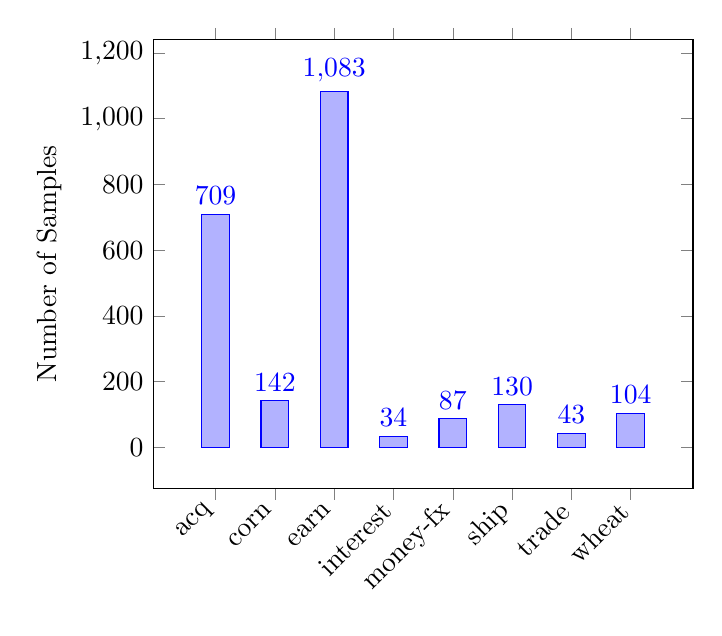
\begin{tikzpicture}
  \begin{axis}[
    ybar,
    enlargelimits=0.15,
    legend style={at={(0.5,-0.2)},
      anchor=north,legend columns=-1},
    ylabel={Number of Samples},
    symbolic x coords={acq,corn,earn,interest,money-fx,ship,trade,wheat},
    xtick=data,
    nodes near coords,
    nodes near coords align={vertical},
    x tick label style={rotate=45,anchor=east},
    ]
    \addplot coordinates {(acq,709) (corn,142)
        (earn,1083) (interest,34) (money-fx,87) (ship, 130) (trade, 43) (wheat, 104)};
  \end{axis}
  \end{tikzpicture}
\end{figure}

The results for each of our feature vectors are: 

\begin{figure}[H]
\centering
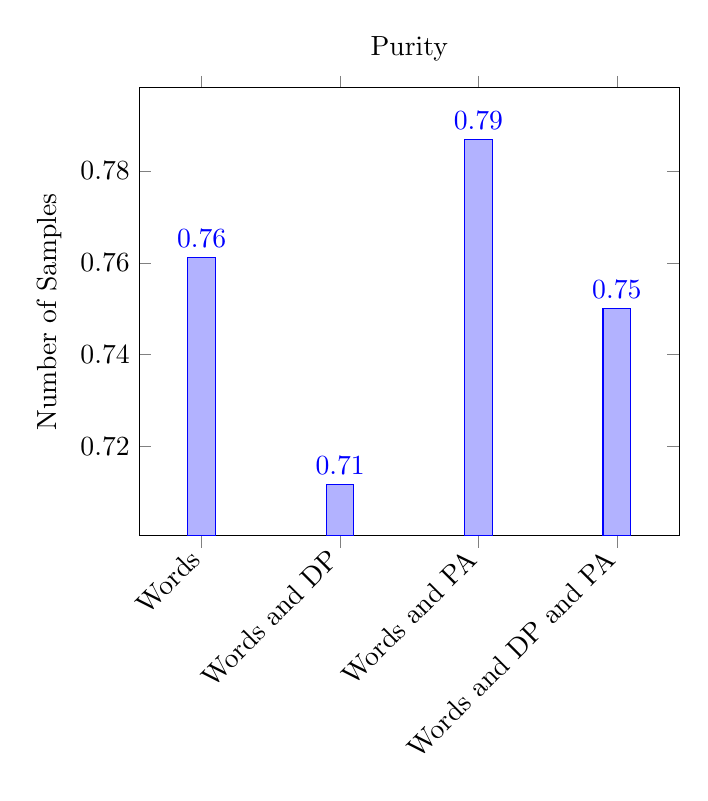
\begin{tikzpicture}
  \begin{axis}[
    ybar,
    enlargelimits=0.15,
    legend style={at={(0.5,-0.2)},
      anchor=north,legend columns=-1},
    ylabel={Number of Samples},
    symbolic x coords={Words,Words and DP,Words and PA,Words and DP and PA},
    xtick=data,
    nodes near coords,
    nodes near coords align={vertical},
    x tick label style={rotate=45,anchor=east},
  title=Purity
    ]
    \addplot coordinates {(Words, 0.761149) (Words and DP,0.711835) (Words and PA,0.786878) (Words and DP and PA,0.75) };
  \end{axis}
  \end{tikzpicture}
\end{figure}

 



 

We evaluate the performance of t


For example, given a corpus of computational linguistics research papers, we might hope that a clustering of the papers would place all the work on grammars and language representations in one cluster, the work on semantics in another, the work in morphology in a third, etc. 

We will reproduce the experiment in \cite{Hurtado2013},  which uses a corpus of 209 artificial intelligence research papers manually tagged by experts. For each paper, the 30 papers considered most similar using the bag-of-words approach \footnote{With tf-idf as the value of the vector for each unigram} with  the cosine distance function were labeled by an expert as similar or dissimilar. A document similarity measure is evaluated by selecting, for each paper, the 30 closest papers and measure the Mean Average Precision and Mean Reciprocal Rank. We will the results of our approach to that of the authors. 

We will also evaluate our document similarity measures on the Reuters-21578 corpus. Each news article in the Reuters corpus is tagged with a class label. We will perform an experiment in which we cluster the articles in the corpus and measure how well each cluster encompasses a class of article and how well each class is represented by a cluster, both in terms of precision and recall. A comparable experiment is done in \cite{Hofmann2000}. 

Finally, if time allows, we will perform an additional experiment on the clustering of research papers, in which we collect a corpus and for each paper return the top $k$ most similar papers. The list of similar papers will then be evaluated by a human subject and the rate of dissimilar papers will be evaluated. 

\subsubsection{Document Classification} \label{sec:DocumentClassification}

The problem of \textbf{document classification} is formally defined just like the general problem of classification in machine learning: Given input pairs of documents and class labels, $(d_1, c_1), (d_2, c_2), \dots, (d_N, c_N)$, with $d_1, \dots d_n \in \mathcal{D}$ and $c_1, \dots, c_N \in \mathcal{C}$, where  $\mathcal{D}$ is the collection of training documents and $\mathcal{C}$ is the set of class labels, assume there is a function $f$ which maps any document $d$ the correct class label $c$. The goal of learning is to approximate the function $f$ with $\hat{f}$ a function created with the observed training data. 

The authors of \cite{Nastase2007} present results from a document classification experiment on the Reuters-21578 dataset using a vector space model which makes use of dependency parsing. We will repeat their experiment to see how our model performs in comparison to theirs. The classification experiment is done using the 10 most frequent classes in the Reuters-21578 document collection with the ModApte split designating the specific documents for training and testing. The precision and recall scores are used to judge the performance of a document similarity measure. 

\subsubsection{Clustering and Classification Methods}

We will use a standard set of machine learning tools to implement the clustering and classification procedures. For clustering, we will perform experiments using \emph{k-means}, \emph{DBSCAN}, and the \emph{EM Algorithm}. For classification, we will perform experiments using \emph{Support Vector Machines}, \emph{Naive Bayes}, and \emph{k-Nearest Neighbor} approaches. We will be programming most of our project in {\tt Python} and will be using the machine learning tools available in {\tt NumPy} and {\tt SciPy}.

\bigskip
\bigskip

\emph{Note the below references includes papers that we read, but did not cite in this document. Those papers are listed for our own reference}.


\nocite{*}

\bibliographystyle{plain}
\bibliography{references}
  
  \end{document}